\section{Background}\label{sec:background}
\subsection{Machine Learning \& Artificial Neural Networks}\label{subsec:machine-learning-and-neural-networks}
Machine learning is a sub-field of artificial intelligence which "provides learning capability to computers
without being explicitly programmed"~\cite{Alzubi_2018}.
More specifically, machine learning allows computers to "learn" patterns and trends from existing data in order to make accurate predictions on new data, without any human input.

Artificial neural networks (ANNs) are a type of machine learning model which draw inspiration from the human brain~\cite{Wang2003}.
These types of models feature "neurons" organized into densely connected layers.
The first layer, which takes in the input data, is known as the input layer while the final layer, which yields the processed output data, is called the output layer.
In between these is at least one hidden layer and in general, having more hidden layers and more neurons per hidden layer allows a neural network to approximate increasingly complex functions.

\begin{figure}[h]
    \centering
    \captionsetup{justification=centering}
    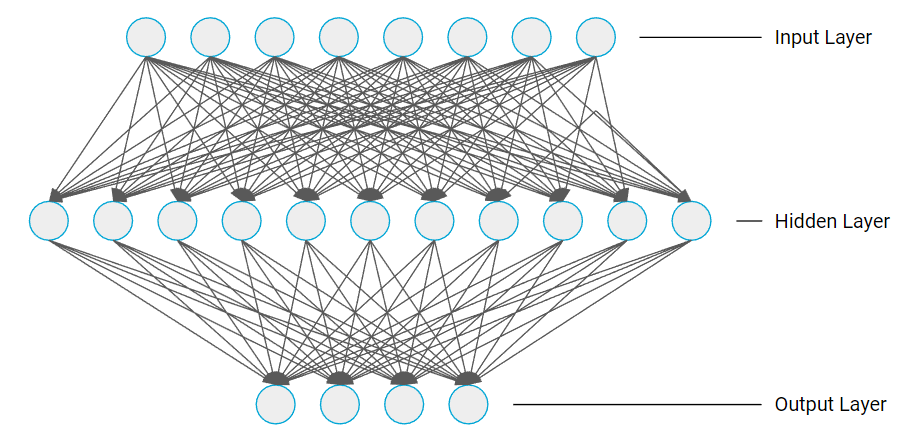
\includegraphics[width=\linewidth]{figures/ann}
    \caption{Visualization of a generic ANN with 8 input neurons and 4 output neurons, as well as a single hidden layer with 11 neurons.}
    \label{fig:ann}
\end{figure}

Each connection between two neurons has an associated weight and bias, which determine how much the output from the source neuron affects the output of the destination neuron.
These values change as the model "learns" from existing data, causing the network's performance to gradually improve.
In addition to this, each neuron passes the combined input of all neurons in the previous layer through a non-linear activation function, which is what allows neural networks to effectively model any function possible~\cite{Wang2003}.

Although ANNs are no longer considered state-of-the-art, understanding the purposes of neurons, neuron connections, layers, and activation functions remains useful, as these still form the building blocks of any neural network architecture.

\subsection{Neural Networks on Embedded Hardware}\label{subsec:machine-learning-on-microcontrollers}
Machine learning, and specifically neural networks, have traditionally been restricted to the realms of high-performance and in turn, high power devices~\cite{8342164}.
Unfortunately, this means that it has been previously impractical to use these technologies with embedded hardware such as microcontrollers, as they lack the memory \& performance to run inference on neural networks locally, while using a remote processor for inference is not always feasible.

However, recent advances into machine learning model compression and optimization have changed this, allowing deep neural networks with multiple hidden layers to be run on devices even powered by coin batteries.
The most prominent development in this field has been TensorFlow Lite for Microcontrollers, which is a Python framework specifically made for optimizing and running neural networks on microcontrollers~\cite{MLSYS2021_d2ddea18}.
This framework introduces two key methods of optimizing neural networks which makes it possible to deploy them on embedded hardware.
The first of these is quantization, which allows converts all 32-bit floating point values and operations in a network to 8-bit integers.
This includes neuron weights, activation functions, input data, and more, resulting in a tremendous improvement to the size of the neural network in memory as well as its runtime.
The second optimization involves loading only the tensor operations that are needed for the neural network.
For example, a neural network might not use any ReLU activation functions or 2D-convolution operations, so these are simply not loaded.

\subsection{Hand Gesture Data}\label{subsec:hand-gesture-data}
In this research, neural networks are used to detect gestures, but to do this, data from some sensor(s) must be fed into the network.

There are a variety of sensors which could be used to record hand gestures and provide this data.
One of these is an accelerometer attached to the user's wrist (typically from a smartwatch) to track the direction and acceleration of the their hand movements~\cite{4912759}.
Another option is using a depth/range camera to record the user's hand, which provides a huge amount of information but in turn requires a computationally intensive video processing pipeline to make sense of the data~\cite{article}.
Photodiodes can also be used, which are sensors that output a signal which increases with the amount of light that hits them.
This means they can track the shadows cast by the user's hand under ambient light, therefore making it possible to recognize which gesture is being performed~\cite{8947919}.
This project uses photodiodes for their much lower monetary and computational cost compared to cameras as well as the fact that they don't require the user to wear a device on their wrists, unlike accelerometers.

\subsection{3D-Formatted Data}\label{subsec:3d-formatted-data}
The term "3D-formatted data" is specific to this research, and must be explained to understand the choice of neural network architectures tested.
This is best done by comparing it to "2D-formatted data".

2D-formatted data can be represented as an image, with some horizontal resolution $x$ and vertical resolution $y$.
In this research, each photodiode outputs values at a predetermined sampling rate over the course of a gesture.
This means that data can be formatted as a 2D image in which $x$ is the number of photodiodes used and $y$ is the number of total samples received from any of the photodiodes.
Therefore, the value of each "pixel" in the image represents a reading from a single photodiode at a single point in time.

3D-formatted data can meanwhile be thought of as a video, which splits this 2D-image into a sequence of $n$ frames, as shown in figure~\ref{fig:3d-data}\@.
3D-formatting is generally more appropriate when the data is sensitive to time, i.e.\ when data points should be considered in a specific sequence.
Therefore, by 3D-formatting the photo diode data, lower error rates should be achievable as temporal information from the photo diodes isn't lost.

\begin{figure}[h]
    \centering
    \captionsetup{justification=centering}
    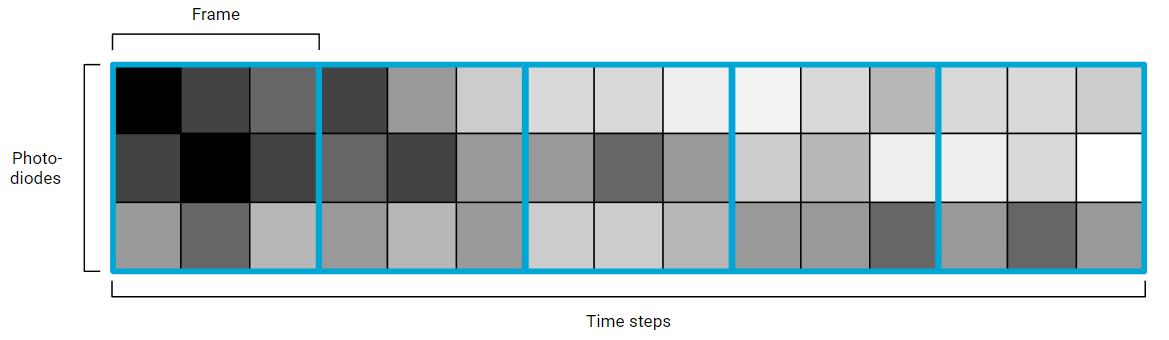
\includegraphics[width=\linewidth]{figures/3d_data}
    \caption{Visualization of 2D photodiode data after being 3D-formatted into 5 frames.}
    \label{fig:3d-data}
\end{figure}